\documentclass[c]{beamer}



\usepackage{tgpagella}
\usepackage[T1]{fontenc}
\usepackage{mdframed}

\setcounter{footnote}{0}

\let\svtikzpicture\tikzpicture
\def\tikzpicture{\noindent\svtikzpicture}
% \usepackage[center]{caption}
\usepackage[caption=false]{subfig}
\usepackage{caption}
\captionsetup{font=small}
\captionsetup[subfigure]{labelformat=empty}
% \usepackage{etex}
% \usepackage[thinc]{esdiff}
% \hyphenation{op-tical net-works semi-conduc-tor}
\usepackage{commath,amsmath,amssymb,amsfonts}
\usepackage{mathtools}
\usepackage{amsthm}
\usepackage{algorithmic}
\usepackage{pgfplots} 
\pgfplotsset{compat=1.15}
\usepackage{graphicx}
\usepackage{pgfgantt}
\usepackage{pdflscape}
\usepackage{pst-plot}
\usepackage{xfrac}
\usepackage{colortbl}
\usepackage{cancel}
\usepgfplotslibrary{fillbetween}
\usepackage{amssymb,bm}
\usepackage{float}
\usepackage{amsmath}
% \usepackage{hyperref}
\usepackage[draft=false]{hyperref}
\usepackage{multirow}
\usepackage{xcolor}
\usepackage{mathrsfs}
\usepackage{bbm}

\usepackage{cite} 

\usepackage{comment}



% \input{tikz-includes.tex}#
%Matlab
% \documentclass{beamer}
\usepackage{xcolor}
\usepackage{listings}
\lstset{ 
	language=Matlab,                		% choose the language of the code
%	basicstyle=10pt,       				% the size of the fonts that are used for the code
	numbers=left,                  			% where to put the line-numbers
	numberstyle=\footnotesize,      		% the size of the fonts that are used for the line-numbers
	stepnumber=1,                   			% the step between two line-numbers. If it's 1 each line will be numbered
	numbersep=5pt,                  		% how far the line-numbers are from the code
%	backgroundcolor=\color{white},  	% choose the background color. You must add \usepackage{color}
	showspaces=false,               		% show spaces adding particular underscores
	showstringspaces=false,         		% underline spaces within strings
	showtabs=false,                 			% show tabs within strings adding particular underscores
%	frame=single,	                			% adds a frame around the code
%	tabsize=2,                				% sets default tabsize to 2 spaces
%	captionpos=b,                   			% sets the caption-position to bottom
	breaklines=true,                			% sets automatic line breaking
	breakatwhitespace=false,        		% sets if automatic breaks should only happen at whitespace
	escapeinside={\%*}{*)}          		% if you want to add a comment within your code
}
%%%%%%%%%%%%%%%%


\usepackage[utf8]{inputenc}
\usepackage{float}
\usepackage{subfigure}
\usepackage{mwe}
\usepackage{trfsigns}
\usepackage{amsmath}
\usepackage{xcolor}
\usepackage{bbm}
% \usepackage{hyperref}
\usepackage{hyperref}
\hypersetup{
    bookmarks=true,         % show bookmarks bar?
    unicode=false,          % non-Latin characters in Acrobat’s bookmarks
    pdftoolbar=true,        % show Acrobat’s toolbar?
    pdfmenubar=true,        % show Acrobat’s menu?
    pdffitwindow=false,     % window fit to page when opened
    pdfstartview={FitH},    % fits the width of the page to the window
    pdftitle={My title},    % title
    pdfauthor={Author},     % author
    pdfsubject={Subject},   % subject of the document
    pdfcreator={Creator},   % creator of the document
    pdfproducer={Producer}, % producer of the document
    pdfkeywords={keyword1, key2, key3}, % list of keywords
    pdfnewwindow=true,      % links in new PDF window
    colorlinks=false,       % false: boxed links; true: colored links
    linkcolor=red,          % color of internal links (change box color with linkbordercolor)
    citecolor=green,        % color of links to bibliography
    filecolor=cyan,         % color of file links
    urlcolor=magenta        % color of external links
}

\lstdefinestyle{mlab}{language=Matlab, numbers=left, numberstyle=\tiny,%5
basicstyle={\ttfamily},%
 keywordstyle={\color{blue}},%
 commentstyle=\color{mlgreen},%
 stringstyle=\color{mlviolett},%
 %breaklines=true,
 }
\lstset{frame=tb,
  language=Java,
  aboveskip=3mm,
  belowskip=3mm,
  showstringspaces=false,
  columns=flexible,
  basicstyle={\small\ttfamily},
  %numbers=none,
  numbers=left,
  numberstyle=\tiny,
  keywordstyle=\color{blue},
  commentstyle=\color{dkgreen},
  stringstyle=\color{mauve},
  breaklines=true,
  breakatwhitespace=true,
  tabsize=3
}


\usepackage{mathrsfs}
%\usepackage{subcaption}
\DeclareMathOperator*{\argmax}{arg\,max}
\DeclareMathOperator*{\argmin}{arg\,min}
% Packages used in LNTthesis class:
% package[english]{babel}   % english language / Englische Sprache
% package{LNTthesis}        % LNT specific definitions / LNT spezifische Definitionen
% package{graphicx}         % for using eps images / Einbinden von EPS Grafiken
% package{verbatim}         % for quickly commenting out large parts of your text / Um viel Text schnell auskommentieren zu koennen
% package{amssymb}          % additional math symbols / Zusaetzliche mathematische Symbole
% package{amsmath}          % additional math commands / Zusaetzliche mathematische Befehle
% package{amsxtra}          % even more math symbols / Noch mehr mathematische Symbole
% package{amsthm}           % theorem environment etc / Theorem Umgebung usw
% more information on amsmath: http://www.ctan.org/get/macros/latex/required/amslatex/math/amsldoc.pdf
% package{psfrag}           % psfrag: http://www.ctan.org/get/macros/latex/contrib/psfrag/pfgguide.pdf
% package{subfigure}        % enable subfigures / Ermoeglicht Subfigures (mehrere Figures neben/untereinander)
% !! PLEASE READ THE LATEX HELP IF YOU HAVE ANY QUESTIONS !!
% http://tobi.oetiker.ch/lshort/lshort.pdf
% Macros:
\newcommand{\eq}[1]{Equation (\ref{#1})}        % \eg{eq:golomb}  --> Equation (2.15)
\newcommand{\eref}[1]{(\ref{#1})}               % \eg{eq:golomb}  --> (2.15)
\newcommand{\fig}[1]{Figure \ref{#1}}           % \fig{fig:golomb}--> Figure 2.15
\newcommand{\tab}[1]{Table \ref{#1}}            % \tab{tab:lala}  --> Table 2.15
\newtheorem{prop}{Proposition}
% Abbreviations
\newcommand{\equivalent}{\triangleq}
\newcommand{\given}{\:\!\vert\:\!}
\usepackage{eucal}

\def \A{\mathcal{A}}
\def \B{\mathcal{B}}
\def \C{\mathcal{C}}
\def \D{\mathcal{D}}
\def \E{\mathcal{E}}
\def \F{\mathcal{F}}
\def \G{\mathcal{G}}
\def \H{\mathcal{H}}
\def \I{\mathcal{I}}
\def \J{\mathcal{J}}
\def \K{\mathcal{K}}
\def \L{\mathcal{L}}
\def \M{\mathcal{M}}
\def \N{\mathcal{N}}
\def \O{\mathcal{O}}
\def \P{\mathcal{P}}
\def \Q{\mathcal{Q}}
\def \R{\mathcal{R}}
\def \S{\mathcal{S}}
\def \T{\mathcal{T}}
\def \U{\mathcal{U}}
\def \V{\mathcal{V}}
\def \W{\mathcal{W}}
\def \X{\mathcal{X}}
\def \Y{\mathcal{Y}}
\def \Z{\mathcal{Z}}
\def \sG {\mathscr{G}}
\def \sU {\mathscr{U}}
\def \sT {\mathscr{T}}
\def \fG{\mathbf{G}}
\def \fa{\mathbf{a}}
\def \fb{\mathbf{b}}
\def \fg{\mathbf{g}}
\def \fu{\mathbf{u}}
\def \fv{\mathbf{v}}
\def \fx{\mathbf{x}}
\def \fy{\mathbf{y}}
\def \fz{\mathbf{z}}
\def \fU{\mathbf{U}}
\def \fV{\mathbf{V}}
\def \fX{\mathbf{X}}
\def \fY{\mathbf{Y}}
\def \fZ{\mathbf{Z}}
\def \f0{\mathbf{0}}
\def \tX{\widetilde{X}}
%
\definecolor{blau_1a}{RGB}{93,133,195}
\definecolor{blau_2a}{RGB}{0,156,218}
\definecolor{gruen_3a}{RGB}{80,182,149}
\definecolor{gruen_4a}{RGB}{175,204,80}
\definecolor{gruen_5a}{RGB}{221,223,72}
\definecolor{orange_6a}{RGB}{255,224,92}
\definecolor{orange_7a}{RGB}{248,186,60}
\definecolor{rot_8a}{RGB}{238,122,52}
\definecolor{rot_9a}{RGB}{233,80,62}
\definecolor{lila_10a}{RGB}{201,48,142}
\definecolor{lila_11a}{RGB}{128,69,151}

% Farbpalette B
\definecolor{blau_1b}{RGB}{0,90,169}
\definecolor{blau_2b}{RGB}{0,131,204}
\definecolor{gruen_3b}{RGB}{0,157,129}
\definecolor{gruen_4b}{RGB}{153,192,0}
\definecolor{gruen_5b}{RGB}{201,212,0}
\definecolor{orange_6b}{RGB}{253,202,0}
\definecolor{orange_7b}{RGB}{245,163,0}
\definecolor{rot_8b}{RGB}{236,101,0}
\definecolor{rot_9b}{RGB}{230,0,26}
\definecolor{lila_10b}{RGB}{166,0,132}
\definecolor{lila_11b}{RGB}{114,16,133}

\definecolor{mycolor1}{rgb}{0.0, 0.18, 0.39}
\definecolor{mycolor2}{RGB}{87,108,67}
\definecolor{mycolor3}{RGB}{8,133,161}
\definecolor{mycolor4}{RGB}{80,91,161}
\definecolor{mycolor5}{RGB}{98,122,157}
\definecolor{mycolor6}{RGB}{255,163,67}
\definecolor{mycolor7}{RGB}{152,205,225}
\definecolor{mycolor8}{RGB}{242,204,48}
\definecolor{mycolor9}{rgb}{0,.5,0}
\definecolor{mycolor10}{rgb}{.59,.44,.09}
%
\definecolor{mycolor11}{RGB}{231,199,31} % Yellow
\definecolor{mycolor12}{RGB}{8,133,161} % Cyan
\definecolor{mycolor13}{RGB}{157,188,64} % Yellow Green
\definecolor{mycolor14}{RGB}{194,150,130} % Light Skin
\definecolor{mycolor15}{RGB}{98,122,157} % Blue Sky
\definecolor{mycolor16}{RGB}{160,160,160} % Neutral
\definecolor{mycolor17}{RGB}{115,82,68} % Dark Skin
\definecolor{mycolor18}{RGB}{94,60,108} % Purple
\definecolor{mycolor19}{RGB}{115,82,68} % Dark Skin
\definecolor{mycolor20}{RGB}{255,183,30} % Dark Gold

\definecolor{mlgreen}{rgb}{.035,.6,.251}
\definecolor{mlviolett}{rgb}{.643,.259,.804}
\definecolor{dkgreen}{rgb}{0,0.6,0}
\definecolor{gray}{rgb}{0.5,0.5,0.5}
\definecolor{mauve}{rgb}{0.58,0,0.82}

\theoremstyle{remark}	\newtheorem{theorem}{Theorem}
\theoremstyle{remark}	\newtheorem{lemma}[theorem]{Lemma}
\theoremstyle{remark}	\newtheorem{corollary}[theorem]{Corollary}
\theoremstyle{remark}	\newtheorem{proposition}[theorem]{Proposition}
\theoremstyle{remark} \newtheorem{definition}{Definition}
\theoremstyle{remark} \newtheorem{remark}{Remark}
\theoremstyle{remark} \newtheorem{example}{Example}
%
\newcommand{\ceil}[1]{\lceil #1 \rceil}
\newcommand{\bigceil}[1]{\Bigl \lceil #1 \Bigr \rceil}
\newcommand{\floor}[1]{\lfloor #1 \rfloor}
\newcommand{\bigfloor}[1]{\Bigl \lfloor #1 \Bigr \rfloor}
%
\usepackage{tikz}
\usepackage{circuitikz}
\usepackage{pgfplots} 
\usepackage{amsmath,amssymb,amsfonts}
\usepackage{commath}
\usepackage{eucal}
\usepackage{mathtools}
\usepackage{amsthm}
\usepackage{algorithmic}
\usepackage{graphicx}
\pgfplotsset{compat=1.15}
\usepackage{graphicx}
\usepackage{capt-of}
\usepackage{lipsum}
\usepackage{float}
\usepackage{pgfgantt}

% \renewcommand{\epsilon}{\varepsilon}
\usepackage{diffcoeff}

\usepackage{autobreak}
\allowdisplaybreaks

% \documentclass{amsart}
\usepackage{mathtools}
\usepackage{tikz}
\usetikzlibrary{positioning}


\usepackage{silence}
\WarningFilter{ctable}{Transparency disabled:}
\usepackage{ctable}

\usepackage{pgfplots}




\usepackage{amsbsy}
\usepackage{bm}
\usepackage{fixmath}

\usepackage{silence}
\WarningFilter{ctable}{Transparency disabled:}
\usepackage{ctable}

\usepackage{pst-node,pst-plot}

\usetikzlibrary{shapes.geometric}

\usepackage{mathdots}

% \usepackage{pgf,tikz}

\usetikzlibrary{math}
\title[Identification Code Via Prime Numbers]{Identification Code Via Prime Numbers}
\author[Emad Zinoghli]{Emad Zinoghli
\vspace{3mm}
\\
\small \text{Institute for Communications Engineering
\hspace{2mm}
\\
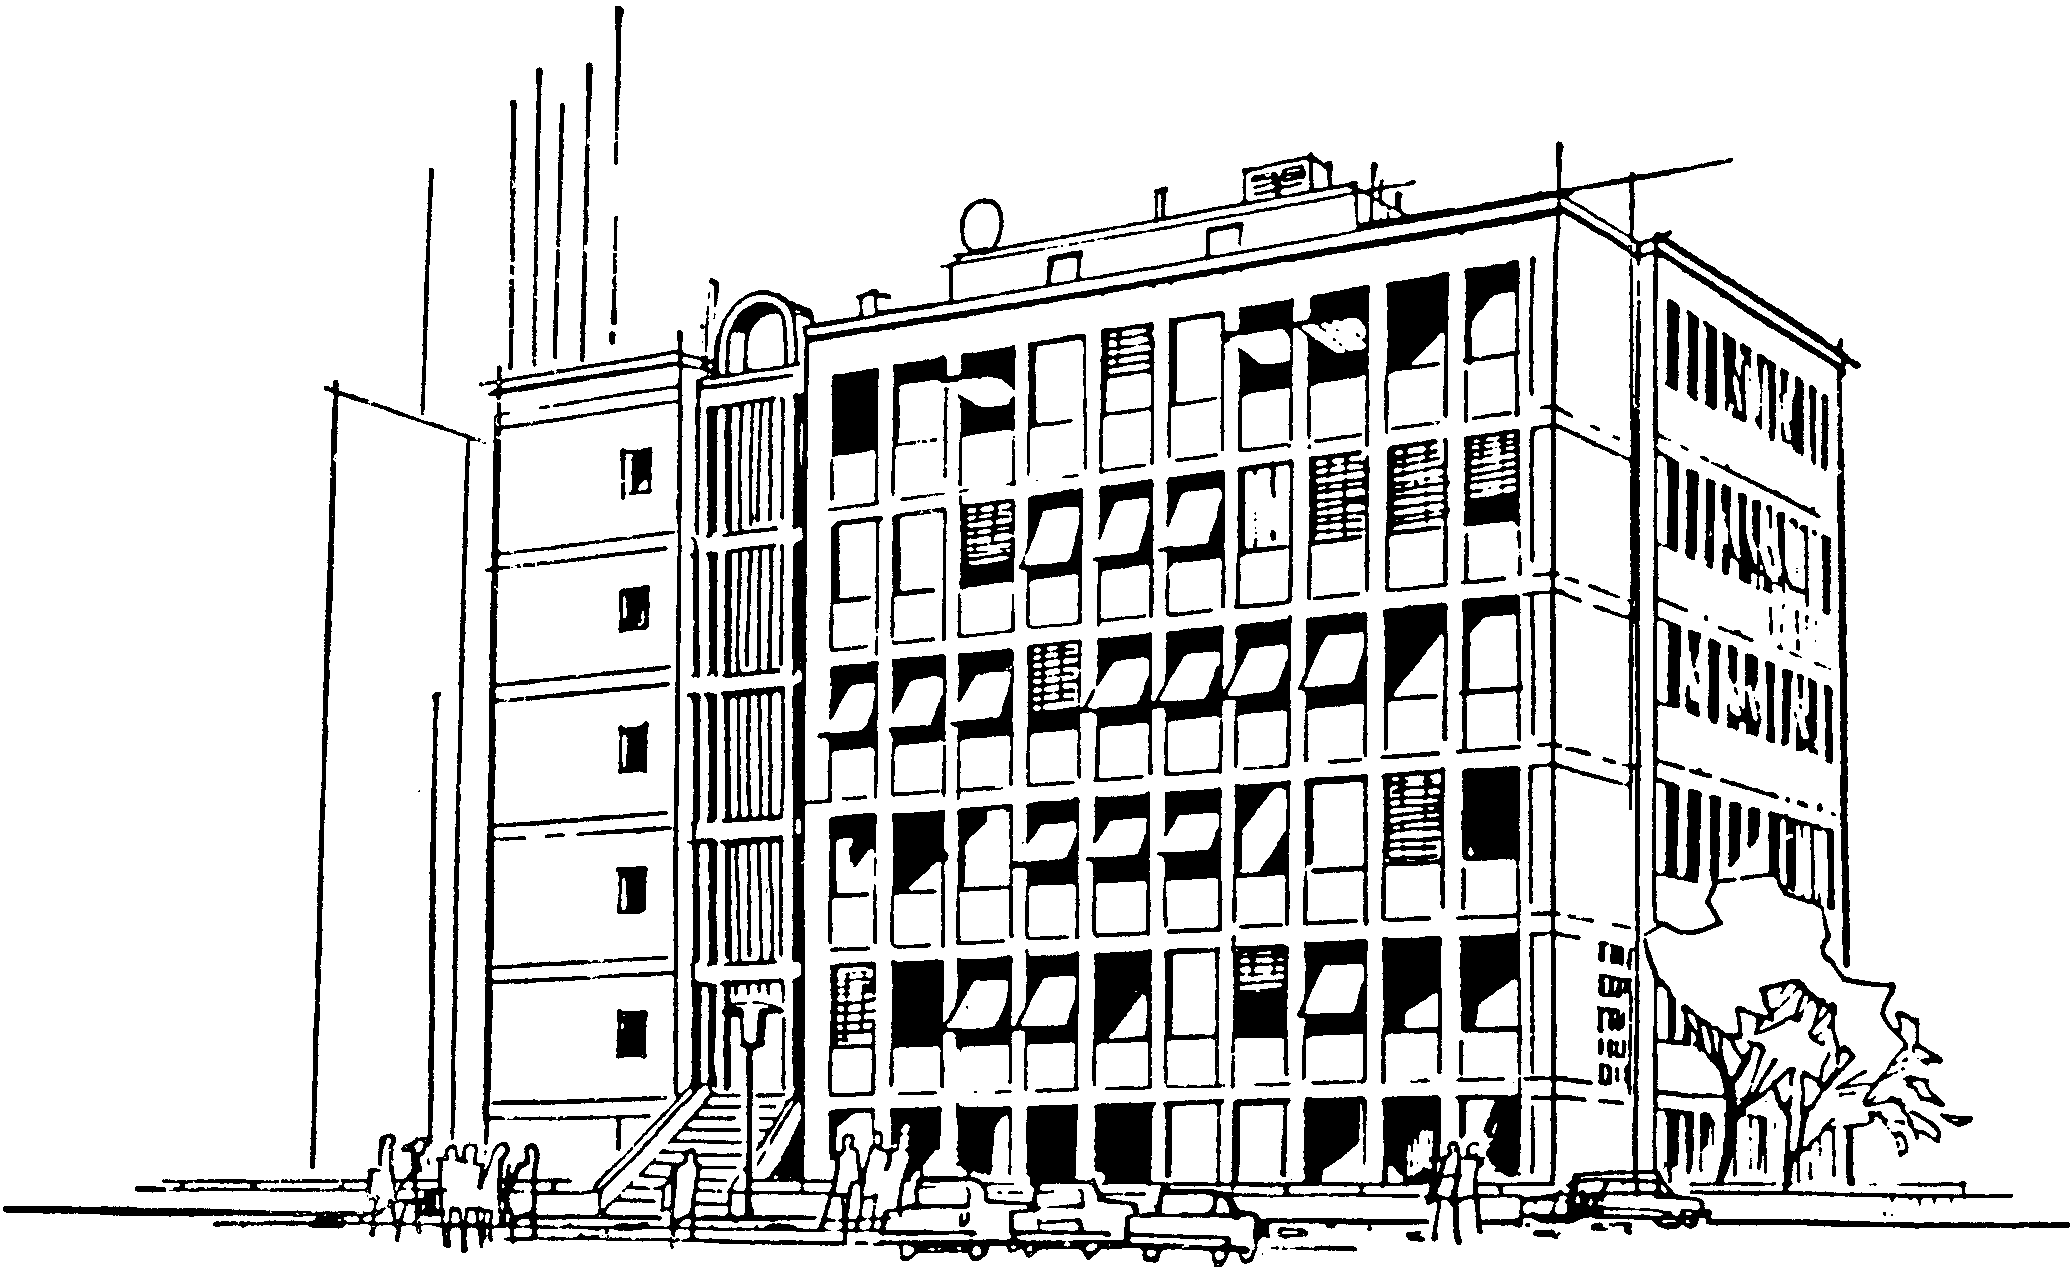
\includegraphics[height = 17mm]{Slides/Fig/N4.png}
}}
\date{March 17, 2022}
\begin{document}
% -----------
\begin{frame}
    \note[item]{Hi everyone.}
	\note[item]{Welcome to my talk.}
	\note[item]{My name is '\textbf{Ons Dabbabi}' and today i will be presenting the result of my \textbf{bachelor thesis}.}
	\note[item]{ with The topic '\textbf{Deterministic Identification For The Binary Symmetric Channel}'.}
	\titlepage 
\end{frame}
% ---------------
\section*{Outline}
\begin{frame}
    \note[item]{I have organized my talk in 5 major topics.}
    \note[item]{In \textbf{Motivation} I establish the concept of identification.}
     \note[item]{In \textbf{Definitions} I provide definitions of Deterministic Identification codes.}
    \note[item]{In \textbf{Main Contributions} the essential contribution to the field is given.}
    \note[item]{In \textbf{Main Results} I present the capacity theorem that I have derived.}
    \note[item]{And finally, I summarize with concluding remarks.}
	\frametitle{Outline}
	\tableofcontents
\end{frame}
% -----------------
\section{Motivation}

\note[item]{Let's focus on the ‘Motivation’.}

\begin{frame}{Transmission vs. Identification}

\note[item]{In the Shannon communication paradigm, in order to transmit a message $i$, Alice employs
a deterministic encoder to select the corresponding Codeword $u_i$.}
\note[item]{Bob, at the decoder side observes a noisy observation of the $u_i$, indicated as vector $Y$.}
\note[item]{Decoder aims to recover the sent message by processing the received vector.}
\note[item]{On the other hand, in the identification scheme proposed by Ahlswede and Dueck, task of the decoder is \textbf{different} is \textbf{not} to estimate the original message.}
\note[item]{In fact, decoder in the identification scheme already has a desired message $j$ and given the observation vector $Y$, it tries to answer a Yes/No question of the following form: \textbf{whether  or not} the original message $i$ is equal to $j$?}
\note[item]{Therefore, decoder output is simply a Yes or No in a reliable form.}

\vspace{4mm}
% \begin{block}{}
    \begin{itemize}
        \item \textcolor{blau_2b}{Shannon's scheme}: Bob recovers the message.
        \vspace{3mm}
        \begin{figure}
        \tikzstyle{farbverlauf} = [ top color=white, bottom color=white!80!gray]
\tikzstyle{block1} = [draw,top color=white, middle color=white!80!orange, rectangle, rounded corners,
minimum height=2em, minimum width=2.5em]

\tikzstyle{block2} = [draw,top color=white, middle color=white!80!orange, rectangle, rounded corners,
minimum height=2em, minimum width=2.5em]

\tikzstyle{block3} = [draw,top color=white, middle color=cyan!30, rectangle, rounded corners,
minimum height=2em, minimum width=2.5em]


\tikzstyle{input} = [coordinate]
\tikzstyle{sum} = [draw, circle,inner sep=0pt, minimum size=5mm,  thick]
\tikzstyle{arrow}=[draw,->]

\begin{tikzpicture}[auto, node distance=2cm,>=latex']
\node[] (M) {$i$};
\node[left=1mm of M] (Alice) {
\includegraphics[height = 14mm]{Fig/Alice.jpg}};
\node[block1,right=.5cm of M] (enc) {Enc};
\node[block3, right=.7cm of enc] (channel) {$\text{\small Channel}$};

\node[block2, right=.7cm of channel] (dec) {Dec};
%\node[below=.5cm of dec] (Target) {$j$};
\node[right=.5cm of dec] (Output) {$\small \hat{i}$};

\node[right=1mm of Output] (Bob) {
\includegraphics[height = 14mm]{Bob.jpg}};

\draw[->] (M) -- (enc);
\draw[->] (enc) --node[above]{$\textbf{u}_i$} (channel);
%\draw[->] (noise) -- (channel);
\draw[->] (channel) --node[above]{$\textbf{Y}$} (dec);

\draw[->] (dec) -- (Output);
%\draw[->] (Target) -- (dec);

% \node[alice, minimum size=.5cm,left = 3mm of M,label=below:{\scriptsize Alice}] (alice) {};
% \node[bob, mirrored, minimum size=.5cm, right=3mm of Output, label=below:{\scriptsize Bob}] (bob) {};

\end{tikzpicture}
        \end{figure}
        \vspace{2mm}
        \item \textcolor{blau_2b}{Identification scheme}: Bob makes a comparison
        \vspace{2mm}
        \begin{figure}
        \tikzstyle{farbverlauf} = [ top color=white, bottom color=white!80!gray]
\tikzstyle{block1} = [draw,top color=white, middle color=white!80!orange, rectangle, rounded corners,
minimum height=2em, minimum width=2.5em]

\tikzstyle{block2} = [draw,top color=white, middle color=white!80!orange, rectangle, rounded corners,
minimum height=2em, minimum width=2.5em]

\tikzstyle{block3} = [draw,top color=white, middle color=cyan!30, rectangle, rounded corners,
minimum height=2em, minimum width=2.5em]


\tikzstyle{input} = [coordinate]
\tikzstyle{sum} = [draw, circle,inner sep=0pt, minimum size=5mm,  thick]
\tikzstyle{arrow}=[draw,->]

\begin{tikzpicture}[auto, node distance=2cm,>=latex']
\node[] (M) {$i$};
\node[left=1mm of M] (Alice) {
\includegraphics[height = 14mm]{Fig/Alice.jpg}};
\node[block1,right=.5cm of M] (enc) {Enc};
\node[block3, right=.7cm of enc] (channel) {$\text{\small Channel}$};

\node[block2, right=.7cm of channel] (dec) {Dec};
\node[below=.5cm of dec] (Target) {$j$};
\node[right=.5cm of dec] (Output) {\text{\small Yes/No}};
\node[right=1mm of Output] (Bob) {
\includegraphics[height = 14mm]{Fig/Bob.jpg}};

\draw[->] (M) -- (enc);
\draw[->] (enc) --node[above]{$\textbf{u}_i$} (channel);
%\draw[->] (noise) -- (channel);
\draw[->] (channel) --node[above]{$\textbf{Y}$} (dec);

\draw[->] (dec) -- (Output);
\draw[->] (Target) -- (dec);

% \node[alice, minimum size=.5cm,left = 3mm of M,label=below:{\scriptsize Alice}] (alice) {};
% \node[bob, mirrored, minimum size=.5cm, right=3mm of Output, label=below:{\scriptsize Bob}] (bob) {};

\end{tikzpicture}
        \end{figure}
    \end{itemize}
% \end{block}
\end{frame}
% --------------
\begin{frame}[c]

\note[item]{Now I compare the standard regime of identification and the K-identification.}
\note[item]{In the standard scenario decoder only check for a comparison, that is, it verifies whether the target
message j equals i or not.}
\note[item]{However for the K-identification, instead of having only one target message in receiver, we have \textbf{K many} messages
and the decoder wants to know if i belongs to this set or not. therefore it only check an inclusion relationship.}
\end{frame} 
% --------------
\begin{frame}[c]
% \vspace{-4mm}
\frametitle{Applications}
% \vspace{1mm}
\only<1>{
\note[item]{Application of deterministic identification includes any event-triggered scenario in which the receiver is not interested to know the \textbf{content} of an event but rather to know \textbf{if} a particular event has happened or not?.}
\note[item]{A second and more concrete example is in distributed computation where two processor aims to check if the two strings that they had coincide or not.}
\note[item]{The olfactory Molecular communication system can also be considered as a good candidate for the deterministic Identification as it is also event triggered in the sense that it detects if a certain smell is present in an environment or not.}
%\note[item]{Furthermore, in the context of communication complexity, two processing unit might wanted to verify whether the Hamming distance of two codewords are the same or not.}
\note[item]{For K-identification, we can consider all the scenarios where receiver wants to spot the presence of an object among a group of objects. Specifically it is used for a more advanced scheme called generalized identification where both the standard and K-identification should be accomplished.}
}
\begin{block}{Standard Deterministic Identification}
    \begin{itemize}
        \item Event triggered systems
        % \footnote{\tiny \textcolor{mycolor2}{Salarisedigh \textit{et al.}, "Deterministic Identification Over Channel With Power Constraints", T-IT, 2021}}
        \item Parallel and distributed computation in VLSI Circuits \footnote{\tiny \textcolor{mycolor2}{J\'aJ\'a, "Information Transfer Under Different Sets of Protocols", SIAM J. Computing, 1984}} \footnote{\tiny \textcolor{mycolor2}{J\'aJ\'a, "Identification is Easier Than Decoding", Proc. Ann. Symp. Found. Comp. Scien.,1985}}
        \item Verification of Hamming distance \footnote{\tiny \textcolor{mycolor2}{R. Paturi, and J. Simon, "Probabilistic Communication Complexity", J. Comput. System Scien., 1986}}
        % \item Pessimistic jamming
        \item Olfactory MC systems (artificial nose) \footnote{\tiny \textcolor{mycolor2}{M. J. Salarisedigh \textit{et al.},, "Deterministic Identification for Molecular Communications over the Poisson Channel", \\ \hspace{6.1mm} arXiv: 2203.02784, 2022}}
    \end{itemize}
\end{block}
%
\vspace{-2mm}
\begin{block}{}
\begin{itemize}
    \item K-Identification $\to$ required in \textcolor{blau_2b}{generalized identification} \footnote{\tiny \textcolor{mycolor2}{R. Ahlswede, "General Theory of Information Transfer: Updated", 2007}} \footnote{\tiny \textcolor{mycolor2}{H. Yamamoto, and M. Ueda, "Multiple Object Identification Coding", T-IT, 2014}}
\end{itemize}
\end{block}
% \pause
% \vspace{-1mm}
% \begin{block}{$K$-Identification}
%     \begin{itemize}
%         \item Perform a local search through objects
        
%     \end{itemize}
% \end{block}
\end{frame}
% --------------
\begin{frame}[c]
\frametitle{Transmission (TR) \footnote{\tiny \textcolor{mycolor2}{C.~E.~Shannon, "A Mathematical Theory of Communication", Bell Sys. Tech. J., 1948}}}

\note[item]{The concept of transmission was introduced in the seminal paper of Shannon in 1948 where he establish a rigorous mathematical
understanding and explanation of the communication problem.}
\note[item]{He derived the capacity of discrete memoryless channel without randomization in the exponential codebook size.}
\note[item]{He showed that for a DMC, the operational capacity equals the information capacity which is maximization of mutual information over the input probabilities.}

\begin{block}{}
    \begin{itemize}
        \item Originally introduced by Shannon (1948)
        \item Capacity was established without randomness at encoder
        \item Decoding sets are disjoint
        \item Codebook size $\textcolor{blau_2b}{\sim 2^{NR}}$
    \end{itemize}
\end{block}
\pause
\begin{theorem}[Shannon, 1948]
    Transmission capacity of a DMC $\W$ in exponential codebook size, i.e., $L(N,R) = 2^{NR}$ is given by
    $$\textcolor{black}{\mathbb{C}_T(\W,L) = \underset{p_X}{\max}~I(X;Y)}$$            
\end{theorem}
\end{frame}
%---------------------------------------------------------
\begin{frame}{Randomized Identification \footnote{\tiny \textcolor{mycolor2}{R. Ahlswede, and G. Dueck, "Identification Via Channels", T-IT, 1989}}}

\only<1>{
\note[item]{The concept of randomized identification was introduced by Ahlswede and Dueck and the capacity was established with randomness at the encoder in the sense
that the encoder use distributions for selection of the Codewords.}
}
\only<2>{
\note[item]{The salient property of this scheme is that reliable identification is possible with for a code size of double exponential in the block-length.}
\note[item]{This is a radical contrast to transmission where the code size is only exponential.}
}
\only<3>{
\note[item]{Ahlswede and Dueck in their seminal paper proved that for DMC the identification capacity and transmission capacity are equal.}
}
% \vspace{1mm}
\begin{block}{}
    \begin{itemize}
        \item Originally introduced by Ahlswede and Dueck (1989)
        \item Capacity was established with randomness at encoder
        \item Encoder employs distribution to select codewords
    \end{itemize}
\end{block}
\pause
\vspace{-2mm}
\begin{block}{Remarkable Property}
\begin{itemize}
    \item Reliable identification is possible with code size growth $\textcolor{blau_2b}{\sim 2^{2^{NR}}}$
    \item Sharp difference to transmission with code size growth $\textcolor{blau_2b}{\sim{2^{NR}}}$
\end{itemize}
\end{block}
\pause
\vspace{-2mm}
\begin{theorem}[Ahlswede and Dueck, 1989]
    RI capacity of a DMC $\W$ in double exponential codebook size, is
    \vspace{.1mm}
    $$\textcolor{black}{\mathbb{C}_{RI}(\W,L = 2^{2^{NR}}) = \underset{p_X}{\max}~I(X;Y)}$$
\end{theorem}
\end{frame}
%------------------------------------------------
\begin{frame}[c]

\note[item]{However for the deterministic regime, encoder uses a deterministic mapping from the messages unto the Codewords.}
\note[item]{deterministic regime is simpler in the implementation and for a DMC it was shown that achievable \textbf{identification} rates are higher than the achievable \textbf{transmission} rates.}

\frametitle{Deterministic Identification (DI) \footnote{\tiny \textcolor{mycolor2}{R. Ahlswede, N. Cai, "Identification Without Randomization", T-IT, 1989}}}
\vspace{2mm}
\begin{block}{}
     \begin{itemize}
     \item Encoder uses deterministic mapping for coding
     \item Simpler Implementation (does not require random resource)
     \item Achievable rates \textbf{higher} than transmission \footnote{\tiny \textcolor{mycolor2}{M. J. Salarisedigh \textit{et al.}, "Deterministic Identification Over Channel With Power Constraints",T-IT, 2022}}
     \end{itemize}
\end{block}
\pause

\only<2>{

\note[item]{When it comes to examine the codebook size of deterministic identification, it is selective, in the sense that
for different discrete or continuous channel it shows different behavior.}
\note[item]{For example, the scale for a DMC is exponential and similar to the transmission scale. However, for the Poisson and Gaussian channels, it was shown recently that the scale is super exponential but still less than the double exponential behavior.}
\note[item]{Unusual scales are already observed in other area such as the covert communication with a scale of sub exponential or covert identification with a codebook size of two to the power of two to the power of $\sqrt{N}R$.}

\vspace{-3mm}
\begin{figure}
    \centering
    \scalebox{.8}{
\begin{tikzpicture}%[remember picture, overlay]
\node (Scale) at (13.3,0) {\text{$L(N,R)$}};
\draw[-{Latex[length=5mm, width=2mm]}] (0,0) -- (12.5,0);
% ---
\node (CC) at (.5,0) {};
\fill [black] (CC) circle (2pt);

\node[rotate = 0] at (.5,.4){\text{$\textcolor{blau_2b!60}{2^{\sqrt{N}R}}$}};

\node[rotate = -20] at (1.7,-.8) {\text{\small \textcolor{blau_2b!60}{Covert Commun.}}};
% ---
\node (TR) at (3,0) {};
\fill [black] (TR) circle (2pt);

\node[rotate = 0] at (3,.4){\text{$\textcolor{blau_2b!70}{2^{NR}}$}};

\node[rotate = -20] at (4,-.7) {\text{\small \textcolor{blau_2b!70}{DI (DMC) \footnote{\tiny \textcolor{mycolor2}{M. J. Salarisedigh \textit{et al.}, "Deterministic Identification Over Channel With Power Constraints", T-IT, 2021}}}}};

% ---
\node (DI) at (5.5,0) {};
\fill [black] (DI) circle (2pt);

\node[rotate = 0] at (5.5,.4){\text{$\textcolor{blau_2b!80}{2^{(N\log N)R}}$}};

\node[rotate = -20] at (7.5,-1) {\text{\small \textcolor{blau_2b!80}{DI (Gaussian \& Poisson) \footnote{\tiny \textcolor{mycolor2}{M. J. Salarisedigh \textit{et al.}, "Deterministic Identification Over Fading Channels", ITW, 2020}} \footnote{\tiny \textcolor{mycolor2}{M. J. Salarisedigh \textit{et al.}, "Deterministic Identification Over Poisson Channels", GC, 2021}}}}};
% ---
\node (CI) at (8,0) {};
\fill [black] (CI) circle (2pt);

\node[rotate = 0] at (8,.4){\text{$\textcolor{blau_2b!90}{2^{2^{\sqrt{N}R}}}$}};

\node[rotate = -20] at (8.7,-.6) {\text{\small \textcolor{blau_2b!90}{Covert ID}}};
% ---
\node (RI) at (10.5,0) {};
\fill [black] (RI) circle (2pt);

\node[rotate = 0] at (10.5,.4){\text{$\textcolor{blau_2b}{2^{2^{NR}}}$}};

\node[rotate = -20] at (11.6,-.8) {\text{\small \textcolor{blau_2b}{Randomized ID}}};

\end{tikzpicture}
}
    \vspace{-3mm}
\end{figure}
}
\end{frame}
%----------------------------------------------------------------
% \begin{frame}[c]
% \frametitle{Deterministic Identification (DI)}
% \begin{block}{Why deterministic?}
% \begin{itemize}
%         \item Simpler Implementation (does not require random resource)
%         \vspace{5mm}
%         \item $\to$ \textbf{Online Sale}
%         \vspace{5mm}
%         \item $\to$ \textbf{Molecular Communication}
%         \begin{itemize}
%             \item Artificial nose
%             \item Target drug delivery and cancer treatment
%         \end{itemize}
%         \vspace{5mm}
%         \item $\to$ \textbf{Pessimistic Jamming}
% \end{itemize}
% \end{block}
% \end{frame}
%--------------------
%\begin{frame}[c]
%\frametitle{Coding Scale Spectrum}
%\begin{figure}
%\input{Slides/Fig/Coding-scale}
%\end{figure}
%\end{frame}
% %------------------------------------------------------------------------------------------------------------------------------------------
\section{Definitions}
\subsection*{DI}
\begin{frame}[c]

\note[item]{A deterministic K-identification code with 5 parameters $M,N,K,\lambda_1$ and $\lambda_2$ for a binary symmetric channel is a system of pairs $(u_i,D_{\S})$ with cardinality $M$ subject to the followings:
\begin{itemize}
    \item $M$ indicate the code-size and is an exponential function of the block-length.
    \item $u_i$ and $D_{\S}$ are Codeword and decoding set respectively.
    \item Target set $\S$ is a subset of input space with size $K$ where itself is again an exponential function of the block-length. We refer to $\kappa$ in the exponent as the identification \textbf{target} rate.
    \item Decoding region is the union of all $\D_i$ where $\D_i$ is the individual decoding region for one specific message $i$.
\end{itemize}}
% \pgfsetfillopacity{1}

\frametitle{K-DI Codes}
\begin{definition}
		An $\textcolor{black}{(M,N,K,\lambda_1,\lambda_2)}$-DI code for BSC $\B$ is a system $\textcolor{black}{\{(\bm{u_i},\mathcal{D}_\mathcal{S})\}_{i\in[1:M]}}$ subject to
            %
            \begin{enumerate}
                \item Codebook size: $M = 2^{NR}$
	            \item Codeword: $\bm{u_i} \in  \mathcal{X}^N$
	            \item Target set $\S\subset [1:M]$ and $|\S|=K=2^{N \kappa}$, where $0\leq\kappa\leq 1$
	            \item Decoding regions: $\mathcal{D}_\S \subset 2^N$, where $\mathcal{D}_\S = \underset{i \in \S}{\bigcup} \mathcal{D}_i$
	            %-----
	            \pgfsetfillopacity{0.2} \item Type I error: $\B^N \left(\mathcal{D}_\S |\bm{u}_i\right) \underset{i \in \S}{\geq} 1-\lambda_1$
	            \pgfsetfillopacity{0.2} \item Type II error: $\B^N \left(\mathcal{D}_\S |\bm{u}_i\right) \underset{i \notin \S}{\leq} \lambda_2$
            \end{enumerate}
            %
\end{definition}
% \pgfsetfillopacity{1}
\end{frame}
% ------------------------
\begin{frame}[c]
\frametitle{K-DI Codes (Cont.)}

\note[item]{Further, there are two error requirements.}
\note[item]{Type I error is similar to that of the standard ID except that it should hold for all target messages.}
\note[item]{Type II error describe the probability of deciding in favor of a message that does not belong to  $\S$.}
\note[item]{For the special case when $K$ is exactly one, we retrieve the standard identification where the $\S$ is a set that includes only one message.}
\begin{definition}
	An $\textcolor{black}{(M,N,K,\lambda_1,\lambda_2)}$-DI code for BSC $\B$ is a system $\textcolor{black}{\{(\bm{u_i},\mathcal{D}_\S))\}_{i\in[1:M]}}$ subject to
            %
            \begin{enumerate}
                \pgfsetfillopacity{0.2} \item Codebook size: $M = 2^{NR}$
	            \pgfsetfillopacity{0.2} \item Codeword: $\bm{u_i} \in 2^N$
	            \pgfsetfillopacity{0.2} \item Target set $\S\subset [1:M]$ and $|\S|=K=2^{N \kappa}$, where $0\leq\kappa\leq 1$
	            \pgfsetfillopacity{0.2} \item Decoding regions: $\mathcal{D}_\S \subset 2^N$, where $\mathcal{D}_\S = \underset{j \in \S}{\bigcup} \mathcal{D}_i$
	            %-----
                 \pgfsetfillopacity{1} \item Type I error: $\B^N \left(\mathcal{D}_\S |\bm{u}_i\right) \underset{i \in \S}{\geq} 1-\lambda_1$
	            \item Type II error: $\B^N \left(\mathcal{D}_\S |\bm{u}_i\right) \underset{i \notin \S}{\leq} \lambda_2$
            \end{enumerate}
            %
\end{definition}
\begin{block}{}
\begin{itemize}
    \item $K=1 \to $ We retrieve the standard identification
\end{itemize}
\end{block}
\end{frame}
% %----------------------------------------
\section{Main Contributions}
\note[item]{Let's now focus on the main contributions that I have derived.}
\begin{frame}[c]
\frametitle{Main Contributions}
\begin{itemize}
\item We derive \textbf{deterministic K-identification} capacity for BSC
\end{itemize}
\end{frame}
% -----------------------
\section{Main Results}
\note[item]{Now we focus on the main results.}
% \begin{frame}[c]
% \frametitle{Proof Minor Mistakes}
% \begin{block}{Mistakes}
% \begin{itemize}
%     % \item $d_{\text{H}}(\fu_{\text{i}},\fu_{\text{j}}) \geq N\beta$ for  $i \neq j$
%     \item Deleting all sequences with $d_{\text{H}}(\fu_{\text{i}},\fu_{\text{j}}) \leq N\beta$
%     \item Decoder subject to $d_{\text{H}}(\fy,\fu_{\text{j}}) \leq N\delta$ 
% \end{itemize}
% \end{block}
% \begin{block}{Solution}
% \begin{itemize}
% %The floor function does not function 
%     \item $d_{\text{H}}(\fu_{\text{i}},\fu_{\text{j}}) \geq \floor{N\beta}+1$ for  $i \neq j$
%     \item Deleting all sequences with $d_{\text{H}}(\fu_{\text{i}},\fu_{\text{j}}) < \floor{N\beta}+1$
%     \item Decoder subject to $d_{\text{H}}(\fy,\fu_{\text{j}}) \leq \floor{N\delta}$ 
% \end{itemize}
% \end{block}
% \end{frame}
%---------------------------
\begin{frame}[c]
\frametitle{DI Over Binary Symmetric Channel}

\note[item]{In this slide you would observe the system model for deterministic identification over the binary symmetric channel with corssover probability $\epsilon$.}
\note[item]{The output of channel is summation of  the input and additive Bernoulli noise with parameter $\epsilon$ in module 2}
\note[item]{Given the observation vector bold vector $\fY$, the task of decoder is to check whether or not the sent message $i$ equals to one of the $K$ elements in the set $\S$ or not.}
\note[item]{We emphasize that before transmission, the sender does not know the set $\S$ otherwise the problem is a degenerate form of transmitting only one bit.}
\begin{figure}
        \tikzstyle{farbverlauf} = [ top color=white, bottom color=white!80!gray]
\tikzstyle{block1} = [draw,top color=white, middle color=white!80!orange, rectangle, rounded corners,
minimum height=2em, minimum width=2.5em]
\tikzstyle{block2} = [draw,top color=white, middle color=white!80!orange, rectangle, rounded corners,
minimum height=2em, minimum width=2.5em]
\tikzstyle{input} = [coordinate]
\tikzstyle{sum} = [draw, circle,inner sep=0pt, minimum size=5mm, thick, color=cyan]
\tikzstyle{arrow}=[draw,->]
\begin{tikzpicture}[auto, node distance=2cm,>=latex']
\node[] (M) {$i$};
\node[block1,right=.5cm of M] (enc) {Enc};
\node[sum, right=2cm of enc] (channel) {$+$};
% \node[below=.5mm of channel] (mod2) {$\text{\scriptsize mod 2}$};
\node[block2, right=2cm of channel] (dec) {Dec};
\node[below=.5cm of dec] (Target) {$\mathcal{S} = \{ j_{\text{1}}, \ldots, j_{\text{K}} \}$};
\node[right=.5cm of dec] (Output) {$\text{\small Yes/No}$};
\node[above=.7cm of channel] (noise) {$\textbf{Z}\sim \text{Ber($\epsilon$)}$};
\draw[->] (M) -- (enc);
\draw[->] (enc) --node[above]{$\textbf{u}_i$} (channel);
\draw[->] (noise) -- (channel);
\draw[->] (channel) --node[above]{$\textbf{Y}$} (dec);
\draw[->] (dec) -- (Output);
\draw[->] (Target) -- (dec);
\end{tikzpicture}

\end{figure}
\begin{block}{}
     \begin{itemize}
        \item $\fY = \fx + \fZ \mod 2$
        \item $Z\sim\text{Bernoulli}(\epsilon)$ for $\epsilon \in (0,\frac{1}{2})$
        \item $\X=\Y=\{0,1\}$
        \item Decoder checks whether $i \in \{ j_1, \ldots, j_K \}$ or not
     \end{itemize}
\end{block}
\end{frame}
% -------------------
\section{Conclusions}
\note[item]{Lets now finalize the talk with some concluding remarks.}
\begin{frame}[c]
\frametitle{Conclusions and Outlook}

\note[item]{As summary I have obtained the K-identification capacity for a binary symmetric channel
and show that one can exhaust asymptotically all the entire input space as for the possible codewords.}
\note[item]{We did some simulation in order to generate an appropriate codebook with the desired Hamming distance property
and obtained a number of curves for the error rates.}
\note[item]{As for the future work, this work can be extended to multi-user scenarios or studying KID problem within the context of generalized identification.}
\note[item]{One can also address an explicit construction of codes when power constraints are imposed.}
    \begin{itemize}
        \item We determine \textbf{deterministic K-ID} capacity of BSC
        \item We observe that correct size for both codebook and target message sets is exponential, i.e., $\textcolor{blau_2b}{\sim{2^{NR}}}$ and $\textcolor{blau_2b}{\sim{2^{N \kappa}}}$
        \item We conduct simulation and analysis of
        \begin{itemize}
            \item Codebook generation and decoding procedure
            \item Type I and II error rates
        \end{itemize}
        \item Future directions
        \begin{enumerate}
                \item DI for multi user scenarios
                % \item Including feedback
                \item Applying K-ID within generalized ID context
                \item Explicit construction code in presence of power constraint
            \end{enumerate}
    \end{itemize}
\end{frame}
% --------------
\begin{frame}[b]
 	\frametitle{Question and Discussion}
 	\vspace{3mm}
    \begin{figure}
    \centering
    
\includegraphics[scale=.43]{Slides/Fig/Q1.jpg}
    \end{figure}
  \vskip30pt
\end{frame}

\end{document}